\documentclass[12pt,a4paper]{report}
\usepackage[english]{babel}
\usepackage[utf8]{inputenc}
\usepackage{fancyhdr}
\usepackage{hyperref}

%Math
\usepackage{amsmath}
\newcommand\norm[1]{\left\lVert#1\right\rVert}
\usepackage{mathtools,xparse}
\usepackage{esvect}
\makeatletter
\newcommand{\leqnomode}{\tagsleft@true\let\veqno\@@leqno}
\newcommand{\reqnomode}{\tagsleft@false\let\veqno\@@eqno}
\makeatother

% graphics
\usepackage{sidecap}
\usepackage{graphicx}
\graphicspath{ {images/} }
% date
\usepackage{datetime}
\newdateformat{specialdate}{\THEYEAR-\twodigit{\THEMONTH}-\twodigit{\THEDAY}}
\date{\specialdate\today}
\usepackage{listings}
\usepackage{xcolor}
\lstset
{ %Formatting for code in appendix
	language=Matlab,
	basicstyle=\footnotesize,
	numbers=left,
	stepnumber=1,
	showstringspaces=false,
	tabsize=2,
	breaklines=true,
	breakatwhitespace=false,
}
\usepackage[miktex]{gnuplottex}  %% I am using miktex

% table of contents
\usepackage{tocloft}

%new commands
\newcommand\tab[1][1cm]{\hspace*{#1}}
\newcommand{\mychapter}[2]{
	\setcounter{chapter}{#1}
	\setcounter{section}{0}
	\chapter*{#2}
	\addcontentsline{toc}{chapter}{#2}
}

%renew commands
\renewcommand{\cftchapleader}{\cftdotfill{\cftdotsep}}
\addto\captionsenglish{% Replace "english" with the language you use
	\renewcommand{\contentsname}%
	{Tabla de contenidos}%
}

\begin{document}
	\begin{titlepage}
		\centering
		
\includegraphics[width=0.2\textwidth]{logo-ugr.png}\\*
		{\scshape\LARGE Universidad de Granada \par}
		{\large \date{\specialdate\today}\par}
		\vspace{1cm}
		{\LARGE\bfseries Los extraños mundos de Belkan\par}
		\vspace{1.5cm}
		{\scshape\large Inteligencia Artificial\par}
		\vspace{2cm}
		{\Large\itshape Lukas Häring García 2ºC\par}
	\end{titlepage}
	\tableofcontents
	\mychapter{0}{Análisis del problema.}
	El objetivo de la práctica es utilizar algoritmos de \textit{búsqueda en grafos}, en esta se recomienda empezar con un algoritmo simple y luego ir cambiando la heurística para optimizarlo.\\*
	He decidido implementar el \textit{algoritmo A*} ya que es una modificación al de búsqueda en anchura.\\*
	\\*
	En este documento voy a explicar los métodos utilizados para solucionar los siguientes problemas:
	\begin{enumerate}
		\item Costo g del algoritmo A*.
		\item Visibilizar área recorrida.
	\end{enumerate}
	\newpage
	\section{Costo g del algoritmo A*.}
	\begin{center}
		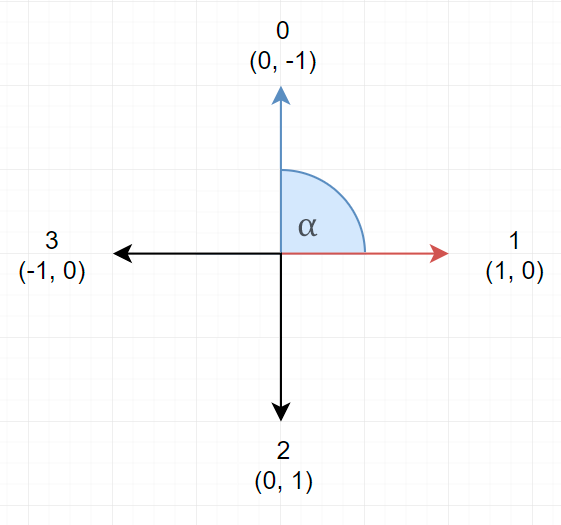
\includegraphics[width=0.5\textwidth]{axis.png}
	\end{center}
	Definimos el vector rojo \textcolor{red}{$\vec{v}$} como la orientación de nuestro personaje y el vector azul \textcolor{blue}{$\vec{w}$}, por lo que el número de giros $\mathbf{T}$ de $90º$ que tiene que dar el vector hasta superponerse ambos. 
	\[
		\textcolor{red}{\vec{v}}+\textcolor{blue}{\vec{w}}=\textcolor{red}{\norm{\vec{v}}}\textcolor{blue}{\norm{\vec{w}}}\cos(\alpha) \Leftrightarrow \textcolor{red}{\vec{v_x}}\textcolor{blue}{\vec{w_x}}+\textcolor{red}{\vec{v_y}}\textcolor{blue}{\vec{w_y}}=\cos(\alpha)
	\]
	Puesto que ambos vectores están normalizados, su módulo es 1, ya que el $\arccos(x)\in\left[-\dfrac{\pi}{2}, \dfrac{\pi}{2}\right]$ el número de vueltas será. 
	\[
		\mathbf{T} = \left\lfloor \dfrac{2}{\pi} \vert\arccos(\textcolor{red}{\vec{v_x}}\textcolor{blue}{\vec{w_x}}+\textcolor{red}{\vec{v_y}}\textcolor{blue}{\vec{w_y}})\vert\right\rfloor \in \{0, 1, 2\}
	\]
	\newpage
	\section{Visibilizar área recorrida.}
	El nivel 3 tiene cierta complejidad puesto que hay que hacer visibles aquellas zonas exploradas una vez encontrado el \textit{punto amarillo}, para ello, yo he optado por una versión más matemática.\\*
	Sea $\theta \in \{0, 90, 180, 270\}$ e $i, j$ las coordenadas del vector que se forma desde la posición $(x,y)$ hasta cada una de las casillas de la imagen, entonces la transformación la ecuación será.\\*
	\begin{figure}[h]
		\centering
		\begin{minipage}{.6\textwidth}
			\[
			\begin{bmatrix}
			\cos(\theta) & -\sin(\theta)\\
			\sin(\theta) & \cos(\theta)
			\end{bmatrix}
			\begin{bmatrix}
			i\\ j
			\end{bmatrix}
			=(1)
			\]
			\[(1)=
			\begin{bmatrix}
			\textcolor{red}{v_x} & -\textcolor{red}{v_y}\\
			\textcolor{red}{v_y} & \textcolor{red}{v_x}
			\end{bmatrix}
			\begin{bmatrix}
			i\\j
			\end{bmatrix}=(2)
			\]
			\[
			(2)=\begin{bmatrix}
			\textcolor{red}{v_x}i-\textcolor{red}{v_y}j)\\\textcolor{red}{v_y}i+\textcolor{red}{v_x}j)
			\end{bmatrix}
			\]
		\end{minipage}%
		\begin{minipage}{.5\textwidth}
			\centering
			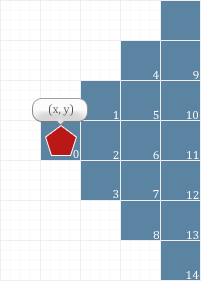
\includegraphics[width=0.7\textwidth]{player_or.png}
		\end{minipage}
	\end{figure}\\*
	Si llevamos esto a código, quedaría lo siguiente.
	\begin{lstlisting}[language=c++]
	int x = /* Posicion X de la entidad. */;
	int y = /* Posicion Y de la entidad. */;
	int bx = /* Coordenada X del Vector Rojo de brujula. */;
	int by = /* Coordenada Y del Vector Rojo de brujula. */;
	for(int j = 0; j < 4; ++j){
		for(int i = -j; i <= -j; ++i){
			int rx = x + (bx * j - by * i);
			int ry = y + (bx * i + by * j);
			mapaResultado[ry][rx] = sensores.terreno[um];
		}
	}
	\end{lstlisting}
	
	\mychapter{3}{Especificaciones}
	\begin{enumerate}
		\item Windows 10.0.14393
		\item Procesador Intel(R) Core(TM) i7-7800X CPU @ 3.50GHz, 3504 Mhz
		\item 6 procesadores principales.
		\item 12 procesadores lógicos.
		\item Memoria física instalada (RAM) 8,00 GB x 2
		\item Compilador MinGW.
	\end{enumerate}

\end{document}